\section{The LHCb experiment}

The LHCb is a dedicated heavy flavor physics experiment situated at the LHC
collider.
The primary purpose of this experiment is searching for new physics in CP
violation and the rare decays of hadrons containing beauty and charm quarks.

This chapter gives a brief overview of the LHCb detector, describes its
subdetectors and their performances. More detailed information and references
on LHCb design and operation can be found in [1].

Firstly the properties of the LHC accelerator are presented, followed by an
overview of the LHCb detector. Then the outline of subdetectors used for
tracking and particle identification is given, followed by the description of
trigger system that is an important part for selecting the most interesting
events while reducing the event rate. Finally, the software used at the LHCb
is described.

\subsection{The LHC}

The Large Hadron Collider (LHC) is a circular proton-proton collider  located
at the European Organization for Nuclear Research (CERN), on the French-Swiss
border, near Geneva. Before the injection of the proton bunches into the main
LHC ring protons pass through series of low-energy pre-accelerators, as shown
in figure~\ref{fig_lhc}.

\begin{figure}[H]
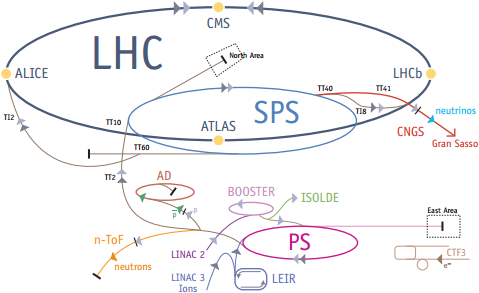
\includegraphics[width=\textwidth]{figs/lhc.png}
\label{fig_lhc}
\caption{The LHC Accelerator System}
\end{figure}

The initial linear accelerator (LINAC2) accelerates protons energy to 50 MeV,
then they are fed through the Proton Synchrotron Booster (BOOSTER) which
accelerates them to 26 GeV, and finally protons are injected  into the LHC
complex at an energy of 450 GeV.

The four main LHC experiments situated at the beam crossing points shown in
figure~\ref{fig_lhc}: ATLAS, ALICE, CMS, LHCb. ALICE dedicated to heavy ion physics.
ATLAS and CMS are general purpose detectors, which primary goal is to discover
production of new particles. More details on the  LHCb experiment, data from
 which is studied in this thesis, are given in the next section.

The new particles are expected to have large masses and their production
processes have small cross sections, so the LHC machine is designed with both
a center-of-mass energy and a luminosity as large as possible.

The operation of the LHC can be shown as follows: two bunch of protons move in
opposite direction in orbit around 27 km circumference of the accelerator by
the magnetic field of superconducting magnets. A temperature 2 K is preserved
for magnets' coils to generate a maximum magnetic field of 8 T.  This field
allows to produce the design center-of-mass energy of $\sqrt{s}=14 TeV$.
Finally the bunches are designed to collide with a frequency of 40 MHz at the
interaction points to archive a design luminosity of $10^{34}cm^{-2}c^{-1}$.

The main LHC design parameters are shown in table~\ref{tab_lhc}. Test

\begin{table}
    \centering
    \begin{tabular}{||r|r||}
      \hline
        Circumference  &  27 km\\
        Center-of-mass energy &  14 TeV\\
        Injection energy  &  450 GeV\\
        Field at 2 $\times$ 450 GeV  &  0.535 T\\
        Field at 2 $\times$ 7 Tev & 8 T\\
        Helium temperature & 2 K\\
        Luminosity & $10^{34}cm^{-2}s^{-1}$\\
        Bunch spacing  & 25 ns\\
        Luminosity lifetime & 10 h\\
        Time between 2 fills  &  7 h\\
      \hline
    \end{tabular}
    \caption{The main LHC design parameters}
\label{tab_lhc}
\end{table}



\subsection{The LHCb}

\subsection{Tracking system}
\subsubsection{Vertex Locater}
\subsubsection{Magnet}
\subsubsection{Inner tracker}
\subsubsection{Outer tracker}

\subsection{Particle identification}
\subsubsection{RICH system}
\subsubsection{Muon system}
\subsubsection{Calorimeter system}

\subsection{Trigger}
\subsubsection{L0 trigger}
\subsubsection{High level trigger}